\documentclass[12pt]{article}
\usepackage[utf8]{inputenc}
\usepackage[margin=1in]{geometry} % Margins
\usepackage{authblk}  % Authors and Affiliations
\usepackage{fancyhdr} % Headers
\usepackage[parfill]{parskip}
\usepackage[inline]{asymptote}
\usepackage{amsmath}
\usepackage{hyperref}
\usepackage{float}
\usepackage{pdfpages}
% \usepackage[t,lf]{spectral}
\usepackage[T1]{fontenc}

\pagestyle{fancy}
\fancyhf{}
\fancyhead[L]{Lavigne du Cadet \& Zhang}
\rhead{\thepage}

\begin{document}
% \includepdf[pages=1]{titlepage.pdf}

\begin{titlepage}
\raggedright

\vspace*{2cm}
% \resizebox{\linewidth}{!}{t-Distributed Stochastic Neighbor Classification Algorithm}

\Huge 
\textbf{t-Distributed Stochastic Neighbor Classification Algorithm}

\vspace{0.5cm}
\small
Quarter 2 Project - \today

\vspace{1.5cm}
\large
\textbf{Jean Lavigne du Cadet} \\
\textbf{Athan Zhang}

\vspace{1cm}
\small
Yilmaz Machine Learning,\\
Thomas Jefferson High School for Science and Technology

\vfill
\large
\textbf{Abstract} \\
\vspace{0.25cm}
\small
Machine learning is a field of artificial intelligence that is concerned with the development of algorithms and models that can learn from and make predictions or decisions without being explicitly programmed. High-dimensional datasets, such as those used in image recognition, are often expensive and time-consuming. This study aims to develop a mathematical model that uses t-Stochastic Neighbor Embedding (t-SNE) combined with classification models to build a cheaper alternative for computer vision uses, while still retaining high accuracy.  We use two of the most widely used datasets for machine learning: the MNIST handwritten digits and CIFAR-10 datasets.
\vspace*{1cm}


\end{titlepage}

\tableofcontents
\newpage

\section{INTRODUCTION}

Machine learning is a field of artificial intelligence that is concerned with the development of algorithms and models that can learn from and make predictions or decisions without being explicitly programmed. It utilizes statistics, mathematics, computer science, and domain-specific knowledge to establish hidden relationships that algorithms can find from data. However, a perpetual limitation in machine learning is the cost of building models around complicated or layered data. 

Datasets with many features, or a high dimensionality, require more resources and time to train models, as well as having a higher chance of having a lower performance. One such example of high dimensional data is image datasets, used for the field of computer vision or image recognition. Convoluted Neural Networks are commonly used to classify these types of datasets, with the ResNet model being famous for its performance and low cost. Nevertheless, this paper aims to develop a more mathematical approach to image classification.

t-Distributed Stochastic Neighbor embedding (t-SNE) is a dimensionality reduction technique commonly used for data visualization as it allows for high dimensional datasets to be reduced to just the second or third dimension, which can be easily turned into visual graphics for a user to see. It “clusters” similar classes with each other visually. It accomplishes this through mathematical techniques that will be covered in Section 2: RELATED WORKS, as well as Section 4: METHODS. This study aims to apply these same concepts for classification, either by applying staple machine learning models to a t-SNE reduced dataset domain or by incorporating classification into the t-SNE algorithm\footnote{ The exact goal of this project has yet to be established, as discussed with Dr. Yilmaz in class. The authors aim to explore how to implement t-SNE for classification but will need to work to figure out how.}.


\section{RELATED WORKS}

The t-SNE algorithm is primarily used for the visualization and transformation of high-dimensionality data and is well-known for being able to map high-dimensional data into 2 dimensions while still maintaining many of the complex relationships \cite{vandermatten2008}. T-SNE is able to maintain the complex relationships due in part to its non-linear nature, stemming from the Gaussian and student-t distributions used.

t-SNE has been benchmarked against several other algorithms, including Sammon Mapping \cite{sammon1969}, Isomap \cite{tenenbaum2000}, and Locally Linearly Embedding \cite{roweis2000}, and also its predecessor, SNE \cite{hinton2002}. These strategies, while they all have their own specific use cases, fail to adequately map image datasets, which will be the primary focus of this paper. For this reason, we selected t-SNE as the principal dimensionality reduction method in our algorithm.
Implementing testing data in our t-SNE algorithm will be a challenge, as the original 2008 paper did not outline a way to classify new data points once the original 2D/3D mapping has been created. To address this problem, researchers have developed ways to embed new data points into an existing t-SNE map \cite{policar2021}. The strategy consists of mapping new similarities between the testing data and reference data in the training set, and subsequently mapping it onto the 2D/3D space, using gradient descent to fine-tune the placement of the points. 

For clustering, several algorithms have been created, including traditional techniques such as k-means \cite{macqueen1967}, hierarchical clustering \cite{johnson1967}, and more recent approaches such as model-based methods \cite{fraley2002}. For our purposes, however, we chose to utilize the density-based clustering method, DBSCAN, for clustering \cite{ester1996}. This is because DBSCAN is able to discover clusters of any size, shape, and density, allowing it to effectively map data points that have been transformed by t-SNE. Moreover, DBSCAN is robust to the presence of noise and outliers, which is often the case in real-world data sets.


\section{DATASET AND FEATURES}

We use two of the most widely used datasets for computer vision machine learning: the MNIST handwritten digits and CIFAR-10 datasets. Table \ref{tab:datasets} provides an overview of the datasets. More information can be found later in this section.

\begin{table}[H]
    \centering
    \begin{tabular}{|c|c|c|c|p{7cm}|}
        \hline
        \textbf{Dataset} & \textbf{Features} & \textbf{Train} & \textbf{Test} & \textbf{Classes}   \\
        \hline
        MNIST & 784 (28 x 28) & 60000 & 10000 & 10 (0-9) \\ 
        CIFAR-10 & 3074 (32 x 32 x 3) & 50000 & 10000 & 10 \newline (airplanes, cars, birds, cats, deer, dogs, frogs, horses, ships, and trucks)\\
        \hline
    \end{tabular}
    \caption{Dataset Information}
    \label{tab:datasets}
\end{table}

\subsection{MNIST}

The MNIST Database of handwritten digit images for machine learning research consists of a collection of handwritten digit images used extensively in optical character recognition and for computer vision machine learning \cite{deng2012}. It’s a modified version of the original National Institute of Standards and Technology database; hence the name modified NIST or MNIST \cite{lecun1998}.

There are 60,000 training images and 10,000 test images, both drawn from the same distribution. The images are black and white, normalized, and centered. The images are 28 by 28 pixels, resulting in the dimensionality of each sample vector being 784 features. The digits 0 through 9 make up the 10 classes. 

\begin{figure}[H]
    \centering
    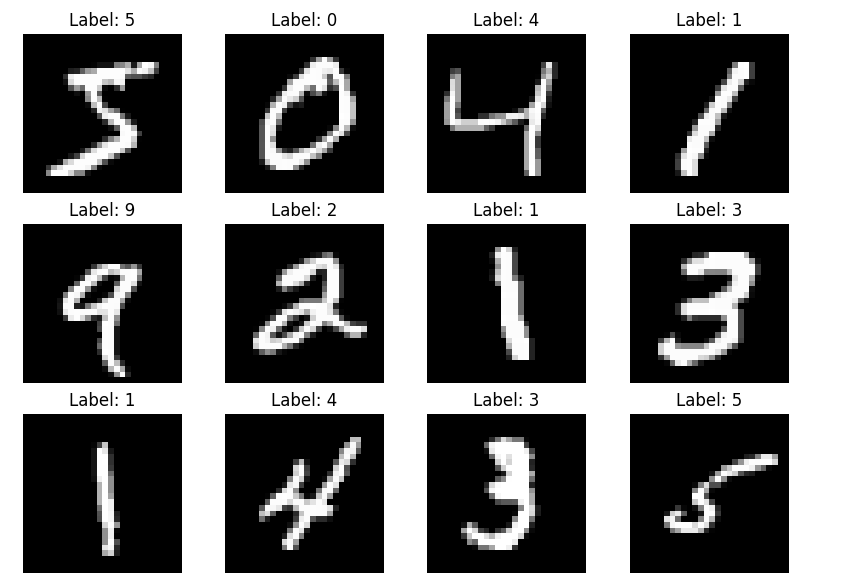
\includegraphics[width=0.8\textwidth]{images/mnist_images.png}
    \caption{Sample Images from the MNIST Dataset}
    \label{fig:mnist_dataset}
\end{figure}

\subsection{CIFAR-10}

The CIFAR-10 dataset, short for Canadian Institute for Advanced Research dataset, is a widely used dataset for image classification tasks. Its primary advantages come from its diversity and challenging nature, making it an ideal dataset for benchmarking and evaluation \cite{krizhevsky2009}.

The dataset consists of 60,000 RGB color images 32 by 32 pixels in size, split into 10 classes with 6,000 images per class. The 10 classes are airplanes, cars, birds, cats, deer, dogs, frogs, horses, ships, and trucks. 

\begin{figure}[H]
    \centering
    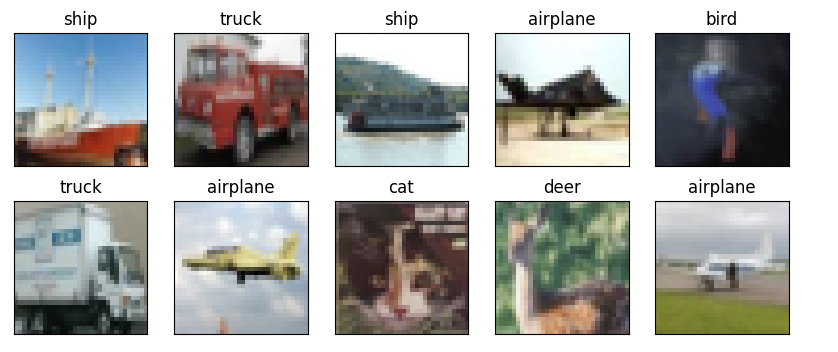
\includegraphics[width=0.8\textwidth]{images/cifar10_images.png}
    \caption{Sample Images from the CIFAR-10 Dataset}
    \label{fig:cifar10_dataset}
\end{figure}


\section{METHODS}

\subsection{t-Distributed Stochastic Neighbor Embedding (t-SNE)}

t-SNE is based on the idea of preserving similarity between points as they go from a high-dimensional space to a low-dimensional (2D, 3D) space. The algorithm begins by constructing a probability distribution for each point in the high-dimensional spaces on a Gaussian distribution, given by the following equation

\begin{align*}
    p_{j|i} = \frac{\exp(-||x_i-x_j||^2/2\sigma_i^2)}{\Sigma_{k\neq{i}}\exp(-||x_i-x_j||^2/2\sigma_i^2)}
\end{align*}

where $\sigma$ is calculated for each point, by conducting a binary search tree until the perplexity of a point matches the perplexity specified by the user. Perplexity is a metric that correlates to the number of neighbors that will have a significant impact on a point’s positioning in the low-dimensional space. The formula given to calculate the perplexity is given by 
\begin{align*}
    Perp(P_i)=2^{H(P_i)}
\end{align*}
\centerline{where}
\begin{align*}
    H(P_i)=1
\end{align*}

Then, the low-dimensional points are initialized randomly. These points are measured in similarity using a student-t distribution which is similar in shape to the Gaussian distribution shown above, but with longer tails:

\begin{align*}
q_{ij} = \frac{(1+||y_i-y_j^2||)^{-1}}{\Sigma_{k\neq{l}}(1+||y_k-y_l||^2)^{-1}}
\end{align*}



Then, gradient descent is performed on the low-dimensional points until an iteration limit is reached or until a local minimum cost has been reached. To determine the derivative cost, which is used to measure how well points are mapped onto the low-dimensional space and to move points in the gradient descent, we use the gradient of Kullback-Leibler divergence, which reduces down to:

\begin{align*}
\frac{\delta C}{\delta y_i} = 2\sum_j (p_{j|i}-q{j|i}+p_{i|j}-q_{i|j})(y_i-y_j)
\end{align*}

Gradient descent is the last stage of the t-SNE algorithm.

\subsection{Classifiers}

Not yet established in the intermediate report…

\subsection{Model Evaluation}

The following metrics were used for the multi-class classification problem previously introduced. The formulas given are a rudimentary derivation of the metric and may deviate slightly from the actual calculated metric used to congregate the multiple classes.

\subsubsection{Accuracy (ACC)}

We use the commonly used classification metric of accuracy (ACC), which is defined by the ratio of the samples correctly classified over the total number of samples.

\begin{align*}
    \text{ACC} = \frac{\text{TP} + \text{TN}}{\text{TP} + \text{TN} + \text{FP} + \text{FN}} \\ 
\end{align*}

\subsubsection{F1-Score (F1)}

F1-Score is the harmonic mean of precision (specificity) and recall (sensitivity). Precision explains how many of the predicted positive cases turned out to actually be positive, while recall explains how many of the actual positive cases the model was able to predict correctly. 

\begin{align*}
    \text{F1} = \frac{2\text{TP}}{2\text{TP} + \text{FP} + \text{FN}} \\ 
\end{align*}

\subsubsection{Area Under Curve (AUC)}

The Area Under the Receiver Operating Characteristic Curve is a commonly used performance metric for evaluating the performance of classification models. It’s calculated by plotting the true positive rate against the false positive rate and then finding the area under the curve formed by the two at different thresholds. The primary advantage of this is that it is insensitive to class imbalance.

\subsection{Implementation}

The proposed approach was implemented on Python 3.6. 

\begin{itemize}
    \item \textbf{Google Drive Folder:}
    \newline \url{https://drive.google.com/drive/folders/1zbz4_EZQ_5hZ2Bo0AcX89MHDQkKk8OBC?usp=share_link}
    
    \item \textbf{Deepnote Workspace:}
    \newline
    \url{https://deepnote.com/workspace/q2-project-athan-and-jean-ac82e86f-be23-4158-8018-cb0aef66aa84/project/MNIST-t-SNE-DTSVMLR-05d74d95-911c-45d1-b339-a9de5574563c}
    
    \item \textbf{GitHub Repository:} 
    \newline
    \textit{In Progress}
\end{itemize}

\section{RESULTS}

Not a part of the intermediate report…

\section{DISCUSSION}

Not a part of the intermediate report…

\section{CONCLUSION}

Not a part of the intermediate report…

\section{AUTHOR CONTRIBUTIONS}

Jean Lavigne Du Cadet (JLDC) and Athan Zhang (AZ) were the primary authors of this paper. Both authors made important contributions to this work. Specifically, JLDC executed literature reviews, model reproduction, and data visualization. AZ conceived and designed the research procedures and experimentation of models. Both authors contributed to drafting the manuscript, reviewing the manuscript, designing the methodology, and analysis.

\section{ACKNOWLEDGEMENTS}

This research did not receive any specific grant from funding agencies in the public, commercial, or not-for-profit sectors. 

The authors would like to thank Dr. Selma Yilmaz of the Thomas Jefferson High School for Science and Technology (TJHSST) for her invaluable contributions in field knowledge and manuscript review.

\bibliographystyle{ieeetr}
\bibliography{refs}

\end{document}